\chapter{Edge AI}
\label{chap:establishing}

\nomenclature{AI}{Artificial Intelligence}
\nomenclature{UAV}{Unmanned Aerial Vehicles}
\nomenclature{WSN}{Wireless Sensor Networks}
\nomenclature{HPS}{Hybrid Pelletized Sinter}
\nomenclature{VANET}{Vehicular Ad Hoc Network}
\nomenclature{ASL}{American Sign Language}
\nomenclature{CNN}{Convolutional Neural Network}
\nomenclature{DNN}{Deep Neural Network}
\nomenclature{LSTM}{Long Short-Term Memory}
\nomenclature{EEG}{Electroencephalography}
\nomenclature{ECG}{Electrocardiography}
\nomenclature{PPG}{Photoplesmiography}
\nomenclature{MCG}{Magnetocardiography}
\nomenclature{FPGA}{Field-Programmable Gate Array}
\nomenclature{MEC}{Mobile Edge Computing}
\nomenclature{HW}{Hardware}
\nomenclature{SW}{Software}
\nomenclature{IDS}{Intrusion Detection System}
\nomenclature{SVM}{Support Vector Machine}

Edge computing has gained several applications in academic, industrial, and commercial media. The fundamental applications of this concept have a vast reach, standing from mobile edge applications to Cloudlets \cite{khan2019edge}. On the one hand, this broad concept creates a large set of possible novel technologies. On the other hand, this vastness requires an organization of the surrounding concepts.

Several novel knowledge areas contribute to the uprise of edge computing. Khan et al. \cite{khan2019edge} enforce that some of these areas are the Internet of Things (IoT), 5G, and augmented reality, among others. They also present a set of several application areas of edge computing, including industrial automation, traffic management, and intelligent monitoring of several environments.

Shi and Dustdar \cite{shi2016promise} suggest that the IoT success has significantly impacted the need for solutions on edge. They discuss that the data processing power of cloud computing is not the only factor to consider when discussing the availability of processing services. Creators should consider that despite the computing power provided by cloud services, some other variables impact the need for edge computing, such as bandwidth and response time.

Satyanarayanan \cite{satyanarayanan2017emergence} also initially assesses the importance of the Internet of Things in the rise of edge computing. The author proposes that the IoT pushed the computing paradigm towards decentralization. The hardware miniaturization contributes to the increased processing power on edge devices. This author reinforces the importance of physical proximity in this context, which is a crucial value when arguing in favor of edge computing appliances.

These discussions show that edge computing is essential in academic and commercial matters. Also, this area is somehow organized, displaying a set of applications in which performing computing on edge is relevant. This text explores how edge computing evolved with artificial intelligence (AI) applications. 

McCarthy \cite{mccarthy2007artificial} described artificial intelligence as the science and engineering to create intelligent machines. In the author's understanding, this intelligence is described as the ability to learn how to achieve goals in the world through an algorithm. The usage of intelligence on edge pursuits to enforce the latest techniques to edge computing scenarios. In the latest years, the most significant advances and breakthroughs are in deep learning, raising a particular interest in performing its integration among different edge computing variations \cite{deng2020edge}.

Before entering the realm of what we will define as Edge AI, it is necessary to choose an edge computing organization as a foundation. In this text, we present a classification similar to Khan et al. \cite{khan2019edge}, which divides edge computing into three main groups:

\begin{itemize}
    \item \textbf{Cloudlets}: In this paradigm, a resourceful infrastructure works similarly to the cloud but are physically near to the end-user;
    \item \textbf{Fog computing}: This paradigm represents virtualization of cloud services to distributed heterogeneous devices closer to the edge of the network;
    \item \textbf{Mobile edge computing}: This perspective considers isolated edge computing networks and services. The local resources and network should provide all the infrastructure.
\end{itemize}

From these three perspectives and concepts, we use these main groups as foundations to describe what Edge AI is and its features. For this matter, Section \ref{sec:defining} will organize and provide a definition for Edge AI, and Section \ref{sec:mapping} will provide an overview of Edge AI applications found in the literature. In Section \ref{sec:taxonomiesanalysis}, we discuss and analyze the main taxonomies for both edge computing and AI, presenting how they contribute to the definitions of Edge Computing assessed above. Finally, we present our proposed taxonomy in Section \ref{sec:taxonomy}, discussing the final aspects and conclusions in Section \ref{sec:conclusions}.

\section{Defining Edge AI}
\label{sec:defining}

In the first section of this text, we presented the relevance of integrating edge computing and AI algorithms. With such an importance, different authors discuss this integration with several names. Some of the names presented in the literature for this confluence are:

\begin{itemize}
    \item Edge Intelligence \cite{deng2020edge,zhou2019edge,liu2020toward};
    \item In-Edge AI \cite{wang2019edge};
    \item Edge AI \cite{li2019edge,lee2018techology};
    \item AI on Edge \cite{greengard2020ai};
\end{itemize}

While other authors discuss the convergence of edge computing and AI without a known name for this phenomenon. Regardless of the name, even in more general discussions, authors usually discuss these concepts within a limited scope of Intelligence algorithms or discuss an aspect of Edge AI/Edge Intelligence.

For instance, Shi et al. \cite{shi2016promise} discuss the communication aspect of Edge AI. Liu et al. \cite{liu2020toward} also discuss the networking and communication aspects. Li et al. \cite{li2019edge} discuss deep learning inference acceleration through edge computing. Zhou et al. \cite{zhou2019edge} present a survey based on deep learning applications in edge computing. Deng et al. \cite{deng2020edge} display an evaluation of the confluence of edge computing and deep learning. Wang et al. \cite{wang2019edge} discuss the convergence of edge computing and AI through federated learning. Although it is natural to overview the most trending AI technologies, the area requires a formal definition that applies to the confluence of artificial intelligence and edge computing regardless of the AI technology.

Concerning the classification of Edge AI devices, Shi et al. \cite{shi2016promise} separate the edge computing elements among two classes: edge devices and edge servers. Then, they discuss the communication-awareness of authors' proposals that developed algorithms and systems based on Edge AI. Their classification can be correlated to the one presented by Khan et al. \cite{khan2019edge}. Mobile edge computing can belong to both edge devices and edge server nodes. Fog computing and cloudlets belong only to the edge server class. Figure \ref{fig:organization} displays a Venn diagram displaying these relationships. The union of these definitions displays a more general classification regarding the works of both authors.

\begin{figure}[ht!]
    \centering
    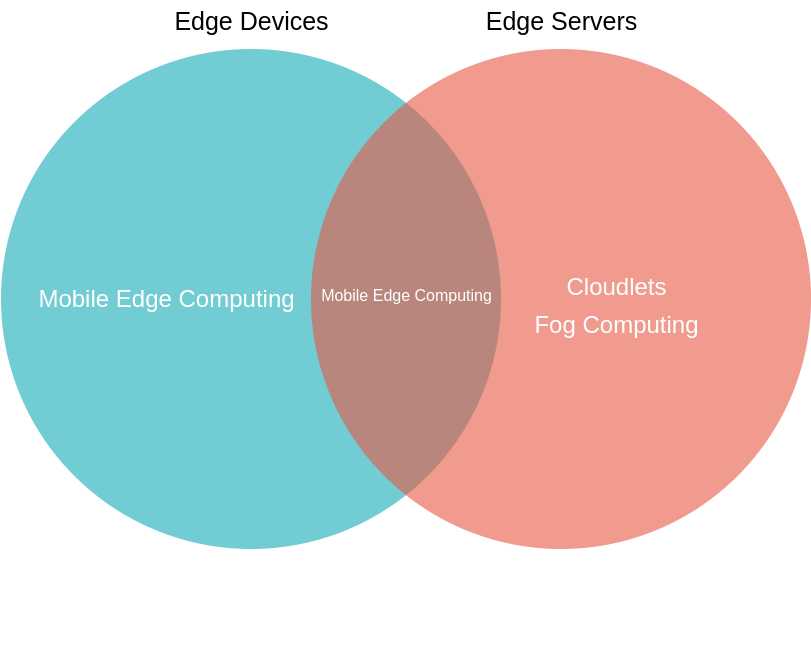
\includegraphics[width = .6\linewidth]{Figures/organization.png}
    \caption{Correspondence to the classifications of edge computing devices and systems from Khan et al. \cite{khan2019edge} and Shi et al. \cite{shi2016promise}}
    \label{fig:organization}
\end{figure}

Regarding a formal Edge AI definition, none of the authors present a formal definition of Edge AI. As much as the definition seems evident at this point, there is no formal sentence defining the concept. For this matter, we establish an entry for the concept of Edge AI.

\begin{itemize}
    \item \textbf{Edge AI Concept:} Edge AI is the set of methods that describes the design process and validation of solutions that combine edge computing and machine learning concepts in developing novel appliances, systems, and applications to solve real-world problems.
\end{itemize}

This definition bases itself on the main common aspects of all evaluated works. It is important to mention that this definition encompasses the other terminologies found in the literature, such as Edge Intelligence, and In-Edge AI, among others. From previous analyses, we also state some of the main features of Edge AI, which are:

\begin{itemize}
    \item Regarding the \textbf{devices' role} in edge computing appliances, the devices can be \textit{edge servers} or \textit{edge devices};
    \item Regarding the \textbf{applications' organization}, an application can be classified among \textit{mobile edge computing}, \textit{fog computing}, and \textit{cloudlets}.
\end{itemize}

We use Edge AI as the official terminology in this work. Nonetheless, it is essential to clarify that this concept and features also refer to works that consider Edge Intelligence or other terminologies, as this is a general terminology. Finally, these terms work regardless of the technologies applied, as long as they can be classified as edge computing and AI together.

\section{Mapping Edge AI applications}
\label{sec:mapping}

After defining the Edge AI, we also provide a mapping of the applications based on this concept. We initially assess and discuss some of the main works regarding Edge AI applications, their organization, and algorithms. Then, we provide some insights on classifying these systems according to the existing organizations and their contexts.

To perform this evaluation, we searched through the bibliography for papers describing applications based on Edge AI. For this matter, we used four different research strings to perform this search, performed on Google Scholar:

\begin{itemize}
    \item ``Edge AI'';
    \item ``Edge Intelligence'';
    \item ``Edge Computing Intelligent System'';
    \item ``Edge AI system'';
\end{itemize}

We initially curated 70 articles describing appliances based on edge computing and AI algorithms. The criteria to select papers was that they should describe one or more case studies that are direct applications of Edge AI. After reviewing this selection, we remained with 54 papers. We excluded those that described general-use frameworks or did not describe specific use cases.

For evaluation purposes, we decided to provide a set of variables to be evaluated considering the edge computing and AI classifications. As discussed in the previous sections, edge computing systems can be classified into three classes according to their organization paradigm: cloudlets, fog computing, or mobile edge computing. Also, the devices running intelligent models can be classified into two main categories: edge devices and edge servers. For the AI, we will initially provide which algorithm or paradigm was used in the appliance. We will also briefly describe the process described in the paper.

\subsection{Applications Overview}

This subsection provides an overview of the applications. Each paragraph describes briefly a single work found in the literature. For each work, we evaluate the system's organization pattern (Mobile Edge, Fog, or Cloudlets), the AI paradigm applied in the solution, and whether the intelligence algorithms run on separate edge servers or edge nodes. The selection and classification criteria are described at the beginning of this section. 

%%%%%%%%%%%%%%%%%%%%%%%%%

The text \textit{iRobot-Factory: An intelligent robot factory based on cognitive manufacturing and edge computing \cite{hu2019irobot}} describes an architecture of a multi-robot factory based on Edge AI. In this case, the edge devices are the robots and sensors involved in the production process. The intelligence algorithms are based on edge servers through direct connection or emulating cloud services. Their application targets the creation of intelligent and integrated industrial architectures.

% \begin{itemize}
%     \item \textbf{Edge computing organization:} Cloudlets;
%     \item \textbf{AI location on edge:} Edge server;
%     \item \textbf{AI paradigms:} Machine Learning, Deep Learning;
% \end{itemize}

%%%%%%%%%%%%%%%%%%%%%%%%%

The work \textit{AI-enabled emotion-aware robot: The fusion of intelligent clothing, edge clouds, and robotics \cite{yang2020ai}} provides a proposal for an application integrating a robot and smart clothing to provide an emotion-aware system to mitigate mental health issues. The involved edge devices, in this case, were wearable devices and robots. Edge server nodes run a system called an emotion-cognition engine to provide AI-based actuation.

% \begin{itemize}
%     \item \textbf{Edge computing organization:} Cloudlets;
%     \item \textbf{AI location on edge:} Edge server;
%     \item \textbf{AI paradigms:} Machine Learning, Deep Learning, Cognitive Computing;
% \end{itemize}

%%%%%%%%%%%%%%%%%%%%%%%%%

The authors of \textit{An edge AI-enabled IoT healthcare monitoring system for smart cities \cite{rathi2021edge}} assess the possibility of creating a healthcare solution based on edge computing, AI, and the IoT. The edge devices involved in this proposal are personal end-users smart devices, patient monitoring devices, and connected ambulances. Intelligent algorithms run on edge servers based in cloudlets.

% \begin{itemize}
%     \item \textbf{Edge computing organization:} Cloudlets;
%     \item \textbf{AI location on edge:} Edge server;
%     \item \textbf{AI paradigms:} Machine Learning, Deep Learning;
% \end{itemize}

%%%%%%%%%%%%%%%%%%%%%%%%%

In \textit{Energy efficient for UAV-enabled mobile edge computing networks: Intelligent task prediction and offloading \cite{wu2020energy}}, the authors provide a network-based application for unmanned aerial vehicles (UAVs) for intelligent tasks. In this work, the edge devices are UAVs, smart devices, and edge servers. The intelligent inferences occur in Edge Servers throughout a mobile edge computing organization. 

% \begin{itemize}
%     \item \textbf{Edge computing organization:} Mobile edge computing;
%     \item \textbf{AI location on edge:} Edge server;
%     \item \textbf{AI paradigms:} Long Short-Term Memory (LSTM)-based prediction, optimization;
% \end{itemize}

%%%%%%%%%%%%%%%%%%%%%%%%%

The work entitled \textit{Real-time strawberry detection using deep neural networks on embedded system (rtsd-net): An edge AI application \cite{zhang2022real}} provides a case study in which the authors apply computer vision and deep neural networks to detect strawberries in real-time. The edge devices involved in this perspective are UAVs and an edge server node. Intelligence algorithms run on the edge server node, provided by the Jetson Nano development board.

% \begin{itemize}
%     \item \textbf{Edge computing organization:} Mobile edge computing;
%     \item \textbf{AI location on edge:} Edge server;
%     \item \textbf{AI paradigms:} Deep Neural Networks (DNNs);
% \end{itemize}

%%%%%%%%%%%%%%%%%%%%%%%%%

In the work named \textit{Edge computing and artificial intelligence for real-time poultry monitoring \cite{debauche2020edge}}, the authors propose and prototype an application for real-time poultry monitoring. The intelligent algorithm runs on a mobile edge computing server based on a Jetson Nano development board. The authors used ESP32 microcontrollers as the media for sensing the environment.

% \begin{itemize}
%     \item \textbf{Edge computing organization:} Mobile edge computing;
%     \item \textbf{AI location on edge:} Edge server;
%     \item \textbf{AI paradigms:} Long Short-Term Memory (LSTM);
% \end{itemize}

%%%%%%%%%%%%%%%%%%%%%%%%%

The text named \textit{Edge AI-IoT pivot irrigation, plant diseases, and pests identification \cite{debauche2020edge-1}} describes the usage of Edge AI within an IoT perspective to detect pests and diseases in plants. They also monitor environmental variables to detect anomalies. In their case, the edge devices are weather stations, remote sensors, and image capturing devices. The edge server runs several intelligent processes to provide insights into understanding environmental health.

% \begin{itemize}
%     \item \textbf{Edge computing organization:} Mobile edge computing;
%     \item \textbf{AI location on edge:} Edge server;
%     \item \textbf{AI paradigms:} Deep Learning;
% \end{itemize}

%%%%%%%%%%%%%%%%%%%%%%%%%

The paper \textit{Edge computing and artificial intelligence for landslides monitoring \cite{elmoulat2020edge}} discusses the possibility of using Wireless Sensor Networks (WSNs), the IoT, and artificial intelligence to monitor landslides. The edge devices involved in the proposed architecture are multiple sensing nodes. The edge servers, in this case, are ODroid N2s and Jetson Nano boards, which run the intelligence algorithms.

% \begin{itemize}
%     \item \textbf{Edge computing organization:} Mobile edge computing;
%     \item \textbf{AI location on edge:} Edge server;
%     \item \textbf{AI paradigms:} Machine Learning;
% \end{itemize}

%%%%%%%%%%%%%%%%%%%%%%%%%

In the article \textit{Edge AI in smart farming IoT: CNNs at the edge and fog computing with LoRa \cite{gia2019edge}} the authors propose an appliance using edge and fog computing to provide Edge AI for smart farming. The edge devices are power-efficient IoT sensors that communicate through LPWAN networks. The intelligence applications are distributed among the fog and cloud layers. 

% \begin{itemize}
%     \item \textbf{Edge computing organization:} Fog computing;
%     \item \textbf{AI location on edge:} Edge server;
%     \item \textbf{AI paradigms:} Long Short-Term Memory (LSTM);
% \end{itemize}

%%%%%%%%%%%%%%%%%%%%%%%%%

In the paper \textit{Edge Intelligence-Assisted Smoke Detection in Foggy Surveillance Environments \cite{muhammad2019edge}}, the authors discuss the training and deployment of an Edge-AI-based system to detect smoke in foggy surveillance environments. The edge intelligence proposed models are convolutional neural networks (CNNs) that classify an image according to the presence of smoke. They search for models with lesser operations per second and size to enable the deployment of edge devices.

% \begin{itemize}
%     \item \textbf{Edge computing organization:} Mobile edge computing;
%     \item \textbf{AI location on edge:} Edge device;
%     \item \textbf{AI paradigms:} Convolutional Neural Networks (CNNs);
% \end{itemize}

%%%%%%%%%%%%%%%%%%%%%%%%%

In the work named \textit{Deep-Learning-Based Visual Odometry Models for Mobile Robotics \cite{de2021deep}}, the authors propose the usage of CNNs and data from a simultaneous localization and mapping (SLAM) data to generate visual odometry models. The edge devices were robots with different capabilities: one can perform slam, while the other relies on visual odometry. The intelligence algorithm runs directly on the edge device.

% \begin{itemize}
%     \item \textbf{Edge computing organization:} Mobile edge computing;
%     \item \textbf{AI location on edge:} Edge device;
%     \item \textbf{AI paradigms:} Convolutional Neural Networks (CNNs);
% \end{itemize}

%%%%%%%%%%%%%%%%%%%%%%%%%

The article \textit{IDiSSC: Edge-computing-based Intelligent Diagnosis Support System for Citrus Inspection \cite{iceis21orange}} presents a proposal of an algorithm to perform the inspection of citrus fruits using Edge AI. The edge devices are image-capturing gear. The authors assess the possibility of using both edge devices or edge server hardware in the disease detection process.

% \begin{itemize}
%     \item \textbf{Edge computing organization:} Mobile edge computing;
%     \item \textbf{AI location on edge:} Edge device or edge server;
%     \item \textbf{AI paradigms:} Machine Learning;
% \end{itemize}

%%%%%%%%%%%%%%%%%%%%%%%%%

In \textit{Conveyor Belt Longitudinal Rip Detection Implementation with Edge AI \cite{Klippel2021}}, the authors assess the proposal of a novel conveyor belt rip detection system using edge AI for the mining industry. The edge devices, in this case, are image-capturing apparatuses. The authors' study considers the possibility of running the intelligence algorithms on both edge devices and edge servers.

% \begin{itemize}
%     \item \textbf{Edge computing organization:} Mobile edge computing;
%     \item \textbf{AI location on edge:} Edge device or edge server;
%     \item \textbf{AI paradigms:} Convolutional Neural Networks (CNNs);
% \end{itemize}

%%%%%%%%%%%%%%%%%%%%%%%%%

The paper \textit{Edge Deep Learning Applied to Granulometric Analysis on Quasi-particles from the Hybrid Pelletized Sinter (HPS) Process \cite{iceis21hps}} discusses a novel proposal for an edge-computing- and AI-based system to detect Quasi-particles in a steel industry process. The edge device involved in this proposal is an image capturing device, which also bears processing capabilities. The intelligence algorithms are CNNs running on the edge device.

% \begin{itemize}
%     \item \textbf{Edge computing organization:} Mobile edge computing;
%     \item \textbf{AI location on edge:} Edge device;
%     \item \textbf{AI paradigms:} Convolutional Neural Networks (CNNs);
% \end{itemize}

%%%%%%%%%%%%%%%%%%%%%%%%%

In the work called \textit{Investigating the Spread of Coronavirus Disease via Edge-AI and Air Pollution Correlation \cite{gomathy2021investigating}}, the authors present an application based on information from an Edge AI system and Air Pollution data to investigate the spread of coronavirus disease. In this case, the authors evaluate the information flow from the cloud to the edge to perform predictions.

% \begin{itemize}
%     \item \textbf{Edge computing organization:} Cloudlets;
%     \item \textbf{AI location on edge:} Edge server;
%     \item \textbf{AI paradigms:} Machine Learning;
% \end{itemize}

%%%%%%%%%%%%%%%%%%%%%%%%%

The paper \textit{A Lossless Data-Hiding based IoT Data Authenticity Model in Edge-AI for Connected Living \cite{rahman2021lossless}} discusses the usage of Edge AI to verify and validate smart living IoT data before passing it through analytics. In this case, the edge devices are local IoT sensor nodes, mainly monitoring the user's health. The intelligent verification algorithm runs on an Edge AI server node.

% \begin{itemize}
%     \item \textbf{Edge computing organization:} Mobile edge computing;
%     \item \textbf{AI location on edge:} Edge server;
%     \item \textbf{AI paradigms:} Ant Colony Optimization;
% \end{itemize}

%%%%%%%%%%%%%%%%%%%%%%%%%

The article \textit{Edge Computing AI-IoT Integrated Energy-Efficient Intelligent Transportation System for Smart Cities \cite{chavhan2022edge}} displays a distributed multi-agent system based on edge computing, AI, and IoT for efficient and intelligent transportation. The intelligence systems run on cloudlets. Edge devices in this network are onboard devices gathering sensor data from transporting agents.

% \begin{itemize}
%     \item \textbf{Edge computing organization:} Cloudlets;
%     \item \textbf{AI location on edge:} Edge server;
%     \item \textbf{AI paradigms:} Stochastic Models, Radial Basis Function Neural Networks;
% \end{itemize}

%%%%%%%%%%%%%%%%%%%%%%%%%

In \textit{National Sports AI Health Management Service System Based on Edge Computing \cite{yang2021national}}, the authors propose an AI sports health management system based on edge computing. Edge devices in this context are smart sensors and intelligent health systems. Intelligence algorithms run in cloudlet layers of the application.

% \begin{itemize}
%     \item \textbf{Edge computing organization:} Cloudlets;
%     \item \textbf{AI location on edge:} Edge server;
%     \item \textbf{AI paradigms:} Query optimization algorithms;
% \end{itemize}

%%%%%%%%%%%%%%%%%%%%%%%%%

The authors of \textit{Towards AI-Based Traffic Counting System with Edge Computing \cite{dinh2021towards}} discuss implementing an AI-based traffic counting system based on the intelligent transportation system concept. The edge devices in this context are cameras capturing live traffic images attached to AI-capable hardware. The edge devices run the intelligence models and feed a server with information.

% \begin{itemize}
%     \item \textbf{Edge computing organization:} Mobile edge computing;
%     \item \textbf{AI location on edge:} Edge device;
%     \item \textbf{AI paradigms:} Convolutional neural networks (CNNs);
% \end{itemize}

%%%%%%%%%%%%%%%%%%%%%%%%%

\textit{Edge AI-Based Automated Detection and Classification of Road Anomalies in VANET Using Deep Learning \cite{bibi2021edge}} discusses the application of DNNs and edge computing to create an intelligent environment for road anomalies detection and classification. Edge devices, in this case, are image-capturing instruments distributed among the network. Edge servers integrate the Vehicular Ad Hoc Network (VANET), running intelligence algorithms.

% \begin{itemize}
%     \item \textbf{Edge computing organization:} Mobile edge computing;
%     \item \textbf{AI location on edge:} Edge server;
%     \item \textbf{AI paradigms:} Deep Neural Networks (DNNs);
% \end{itemize}

%%%%%%%%%%%%%%%%%%%%%%%%%

The work named \textit{Intelligent and Smart Irrigation System Using Edge Computing and IoT \cite{munir2021intelligent}} proposes the intelligent usage of ontology and sensor data together with a machine learning classification algorithm to create a smart irrigation system based on Edge AI. Edge devices are smart sensors capturing field data. Intelligent algorithms run on the edge server layer.

% \begin{itemize}
%     \item \textbf{Edge computing organization:} Mobile edge computing;
%     \item \textbf{AI location on edge:} Edge server;
%     \item \textbf{AI paradigms:} Machine Learning;
% \end{itemize}

%%%%%%%%%%%%%%%%%%%%%%%%%

The paper entitled \textit{AI at the Edge for Sign Language Learning Support \cite{battistoni2019ai}} suggests a novel method to recognize the American Sign Language (ASL) alphabet using CNNs and Fog Computing. Edge devices in this architecture are smart end devices responsible for capturing images. The proposed method deploys the intelligent algorithms on a fog computing layer.

% \begin{itemize}
%     \item \textbf{Edge computing organization:} Fog computing;
%     \item \textbf{AI location on edge:} Edge server;
%     \item \textbf{AI paradigms:} Convolutional Neural Networks (CNNs);
% \end{itemize}

%%%%%%%%%%%%%%%%%%%%%%%%%

In \textit{AI on edge device for laser chip defect detection \cite{hou2019ai}}, the authors propose a novel edge system to detect defects in chips based on laser images. Intelligence algorithms run on the edge device, accelerated by a neural network stick. The edge devices are computer-on-modules with an attached microscope and a neural network accelerator.

% \begin{itemize}
%     \item \textbf{Edge computing organization:} Mobile edge computing;
%     \item \textbf{AI location on edge:} Edge device;
%     \item \textbf{AI paradigms:} Convolutional Neural Networks (CNNs);
% \end{itemize}

%%%%%%%%%%%%%%%%%%%%%%%%%

The work \textit{An AI-edge Platform with Multimodal Wearable Physiological Signals Monitoring Sensors for Affective Computing Applications \cite{yang2020ai-2}} displays a proposal for a novel platform to monitor user's emotions. The edge devices are a set of wearable sensors measuring electroencephalography (EEG), electrocardiography (ECG), and photoplesmiography (PPG). Intelligence algorithms run on an AI/IoT edge server based on FPGA and a RISC-V platform.

% \begin{itemize}
%     \item \textbf{Edge computing organization:} Mobile edge computing;
%     \item \textbf{AI location on edge:} Edge server;
%     \item \textbf{AI paradigms:} Convolutional Neural Networks (CNNs);
% \end{itemize}

%%%%%%%%%%%%%%%%%%%%%%%%%

In \textit{A New Deep Learning-Based Food Recognition System for Dietary Assessment on An Edge Computing Service Infrastructure \cite{liu2017new}}, the authors propose a food recognition system based on edge computing and AI. Edge devices in this proposal are mobile image capturing devices. The intelligent processing happens in a cloudlet layer.

% \begin{itemize}
%     \item \textbf{Edge computing organization:} Cloudlets;
%     \item \textbf{AI location on edge:} Edge server;
%     \item \textbf{AI paradigms:} Convolutional Neural Networks (CNNs);
% \end{itemize}

%%%%%%%%%%%%%%%%%%%%%%%%%

The authors of \textit{Implementation of Pavement Defect Detection System on Edge Computing Platform \cite{lin2021implementation}} present a novel edge computing platform to detect defects in pavements. Edge devices are a composition of cameras and computing modules. Intelligence algorithms run on these specialized modules, which can be computer-on-modules or FPGAs.

% \begin{itemize}
%     \item \textbf{Edge computing organization:} Mobile edge computing;
%     \item \textbf{AI location on edge:} Edge device;
%     \item \textbf{AI paradigms:} Convolutional Neural Networks (CNNs);
% \end{itemize}

%%%%%%%%%%%%%%%%%%%%%%%%%

\textit{Edge-AI-Based Real-Time Automated License Plate Recognition System \cite{lin2022edge}} presents a new license plate recognition system based on Edge AI and IoT. The edge intelligence runs on the device, which has AI accelerators. The edge devices are image-capturing computer-on-modules.

% \begin{itemize}
%     \item \textbf{Edge computing organization:} Mobile edge computing;
%     \item \textbf{AI location on edge:} Edge device;
%     \item \textbf{AI paradigms:} Convolutional Neural Networks (CNNs);
% \end{itemize}

%%%%%%%%%%%%%%%%%%%%%%%%%

In \textit{A Wireless Multi-Channel Capacitive Sensor System for Efficient Glove-Based Gesture Recognition With AI at the Edge \cite{pan2020wireless}}, the authors present a wearable-based edge system for ASL gesture recognition. Their edge device is a wearable system based on capacitive sensors. The edge intelligence runs in the wearable computer-on-module.

% \begin{itemize}
%     \item \textbf{Edge computing organization:} Mobile edge computing;
%     \item \textbf{AI location on edge:} Edge device;
%     \item \textbf{AI paradigms:} Machine Learning;
% \end{itemize}

%%%%%%%%%%%%%%%%%%%%%%%%%

\textit{Blockchain-Based Trust Edge Knowledge Inference of Multi-Robot Systems for Collaborative Tasks \cite{li2021blockchain}} provides a proposal for a blockchain-based system to provide AI inferences in multi-robot systems. Edge devices are robots composing a multi-robot system. Edge servers, in this case, are local Edge AI nodes that run AI inference algorithms.

% \begin{itemize}
%     \item \textbf{Edge computing organization:} Cloudlets;
%     \item \textbf{AI location on edge:} Edge server;
%     \item \textbf{AI paradigms:} Machine Learning;
% \end{itemize}

%%%%%%%%%%%%%%%%%%%%%%%%%

The paper \textit{Deep Learning Models for Magnetic Cardiography Edge Sensors Implementing Noise Processing and Diagnostics \cite{sakib2021deep}} presents an implementation of deep learning models to process noise and aid in diagnostics using magnetic cardiography edge sensors. Edge devices, in this case, are magnetocardiography (MCG) sensors. Signals are processed in a high-performance edge machine as an edge server.

% \begin{itemize}
%     \item \textbf{Edge computing organization:} Cloudlets;
%     \item \textbf{AI location on edge:} Edge server;
%     \item \textbf{AI paradigms:} Deep Learning;
% \end{itemize}

%%%%%%%%%%%%%%%%%%%%%%%%%

In the work \textit{Deep Reinforcement Learning for Collaborative Edge Computing in Vehicular Networks \cite{li2020deep}}, the authors display a mobile edge computing system based on collaborative and decentralized intelligence in vehicular applications. Edge devices are onboard computers in vehicular networks. Edge servers are distributed edge clusters that run the intelligence algorithms.

% \begin{itemize}
%     \item \textbf{Edge computing organization:} Mobile edge computing;
%     \item \textbf{AI location on edge:} Edge server;
%     \item \textbf{AI paradigms:} Convolutional Neural Networks (CNNs);
% \end{itemize}

%%%%%%%%%%%%%%%%%%%%%%%%%

The work named \textit{Development and Validation of an EEG-Based Real-Time Emotion Recognition System Using Edge AI Computing Platform With Convolutional Neural Network System-on-Chip Design \cite{fang2019development}} displays a solution to recognize emotions using electroencephalography (EEG) data. The edge device employed in this system is a field-programmable gate array (FPGA) board. For the edge server, the application uses networking to develop high-level appliances using the inferences from the edge devices.

% \begin{itemize}
%     \item \textbf{Edge computing organization:} Mobile edge computing;
%     \item \textbf{AI location on edge:} Edge device;
%     \item \textbf{AI paradigms:} Convolutional Neural Networks (CNNs);
% \end{itemize}

%%%%%%%%%%%%%%%%%%%%%%%%%

In the article \textit{Distributed Deep Learning Model for Intelligent Video Surveillance Systems with Edge Computing \cite{chen2019distributed}}, the authors propose a novel model for video surveillance systems based on Edge AI. These are two layers of edge servers, organized as a mobile edge computing appliance and getting closer to cloud integration. In this context, the edge devices are video capturing devices.

% \begin{itemize}
%     \item \textbf{Edge computing organization:} Mobile edge computing;
%     \item \textbf{AI location on edge:} Edge device;
%     \item \textbf{AI paradigms:} Convolutional Neural Networks (CNNs) and Long Short-Term Memory (LSTM);
% \end{itemize}

%%%%%%%%%%%%%%%%%%%%%%%%%

\textit{Edge-AI in LoRa-based Health Monitoring: Fall Detection System with Fog Computing and LSTM Recurrent Neural Networks \cite{queralta2019edge}} presents the proposal of an ecosystem based on Edge AI and LPWAN connections toward remote healthcare monitoring. The edge devices are wearable IoT sensors. Edge servers provide the intelligence algorithms necessary to analyze signals and detect falls.

% \begin{itemize}
%     \item \textbf{Edge computing organization:} Fog computing;
%     \item \textbf{AI location on edge:} Edge server;
%     \item \textbf{AI paradigms:} Long Short-Term Memory (LSTM);
% \end{itemize}


%%%%%%%%%%%%%%%%%%%%%%%%%

The article \textit{Edge artificial intelligence for the industrial internet of things applications: an industrial edge intelligence solution \cite{foukalas2021edge}} presented a novel edge-computing-based model for developing intelligent industrial solutions. The edge devices present in this work are industrial end devices performing several tasks. The intelligence models are updated in the edge servers within the federated learning organization.

% \begin{itemize}
%     \item \textbf{Edge computing organization:} Cloudlets;
%     \item \textbf{AI location on edge:} Edge device;
%     \item \textbf{AI paradigms:} Federated Learning;
% \end{itemize}

%%%%%%%%%%%%%%%%%%%%%%%%%

\textit{AI-Aided Individual Emergency Detection System in Edge-Internet of Things Environments \cite{yang2021ai}} displays an innovative individual emergency detection system based on IoT and edge intelligence. The edge devices, in this case, are mobile phones, capturing their sensors' data throughout the usage time. The intelligence models run on edge servers. 

% \begin{itemize}
%     \item \textbf{Edge computing organization:} Mobile edge computing;
%     \item \textbf{AI location on edge:} Edge server;
%     \item \textbf{AI paradigms:} Multi-layer perceptron (MLP), Support vector machine (SVM), Convolutional neural networks (CNNs);
% \end{itemize}

%%%%%%%%%%%%%%%%%%%%%%%%%

In \textit{Economic data analytic AI technique on IoT edge devices for health
monitoring of agriculture machines \cite{gupta2020economic}}, the authors provide a novel integration model for agricultural machines using Edge AI. In their case, the edge devices are agriculture machines (AgMs) producing data from interconnected sensors. Edge servers run in distributed mobile devices which perform inferences using lightweight models.

% \begin{itemize}
%     \item \textbf{Edge computing organization:} Mobile edge computing;
%     \item \textbf{AI location on edge:} Edge server;
%     \item \textbf{AI paradigms:} Artificial neural networks (ANN);
% \end{itemize}

%%%%%%%%%%%%%%%%%%%%%%%%%

In the article named \textit{Intelligent Edge Computing for IoT-Based Energy Management in Smart Cities \cite{liu2019intelligent}}, the authors present a design for an Edge-AI-based energy management system. In their perspective, the edge devices are IoT sensors distributed on the network. Mid-term edge servers provide intelligent services for energy management.

% \begin{itemize}
%     \item \textbf{Edge computing organization:} Cloudlets;
%     \item \textbf{AI location on edge:} Edge server;
%     \item \textbf{AI paradigms:} Deep neural networks (DNN);
% \end{itemize}

%%%%%%%%%%%%%%%%%%%%%%%%%

\textit{Intelligent Search and Find System for Robotic Platform Based on Smart Edge Computing Service \cite{barnawi2020intelligent}} displays a novel edge service to provide intelligent task division algorithms. The edge devices in this perspective are autonomous robots. A base station contains a terminal that provides a self-design intelligence algorithm and interfaces with an operator. 

% \begin{itemize}
%     \item \textbf{Edge computing organization:} Mobile edge computing;
%     \item \textbf{AI location on edge:} Edge server;
%     \item \textbf{AI paradigms:} Traversal Algorithm;
% \end{itemize}

%%%%%%%%%%%%%%%%%%%%%%%%%

In the article named \textit{Intelligent Traffic Accident Detection System Based on Mobile Edge Computing \cite{liao2017intelligent}}, the authors display a traffic accident detection system based on Edge AI. The edge devices within this perspective are smartphones within a mobile edge computing (MEC) network. Mobile edge servers provide the intelligence algorithms as a service.

% \begin{itemize}
%     \item \textbf{Edge computing organization:} Mobile edge computing;
%     \item \textbf{AI location on edge:} Edge server;
%     \item \textbf{AI paradigms:} Deep neural networks (DNN);
% \end{itemize}

%%%%%%%%%%%%%%%%%%%%%%%%%

The authors of \textit{Low-Power HW Accelerator for AI Edge-Computing in Human Activity Recognition Systems \cite{de2020low}} propose an efficient hardware-accelerated system for human activity recognition. The edge device in this context is self-developed hardware to read inertial sensors and processes. The edge intelligence algorithms are hardware accelerated hybrid neural networks.

% \begin{itemize}
%     \item \textbf{Edge computing organization:} Mobile edge computing;
%     \item \textbf{AI location on edge:} Edge device;
%     \item \textbf{AI paradigms:} Hybrid neural networks (HNN);
% \end{itemize}

%%%%%%%%%%%%%%%%%%%%%%%%%

In the article named \textit{pAElla: Edge AI-Based Real-Time Malware Detection in Data Centers \cite{libri2020paella}}, the authors propose a lightweight and scalable solution to monitor the presence of malware in data centers. The intelligence algorithms are designed to run in the edge devices, which feed inferences to an edge server. The edge devices are IoT computer-on-modules based on ARM processors.

% \begin{itemize}
%     \item \textbf{Edge computing organization:} Mobile edge computing;
%     \item \textbf{AI location on edge:} Edge device;
%     \item \textbf{AI paradigms:} Convolutional Neural Networks (CNNs);
% \end{itemize}

%%%%%%%%%%%%%%%%%%%%%%%%%

The paper \textit{Passban IDS: An Intelligent Anomaly-Based Intrusion Detection System for IoT Edge Devices \cite{eskandari2020passban}} displays a novel IoT intrusion detection system (IDS) based on smart edge computing. The edge devices in this context are IoT gateways. Machine learning models on these gateways provide predictions of potentially hazardous packages.

% \begin{itemize}
%     \item \textbf{Edge computing organization:} Mobile edge computing;
%     \item \textbf{AI location on edge:} Edge device;
%     \item \textbf{AI paradigms:} Machine Learning;
% \end{itemize}

%%%%%%%%%%%%%%%%%%%%%%%%%

\textit{Real-Time Apple Detection System Using Embedded Systems With Hardware Accelerators: An Edge AI Application \cite{mazzia2020real}} presents a novel system to detect apples in orchards based on Edge AI devices. For edge devices, the authors propose several solutions based on embedded computers. These computers run intelligent models to detect the apples directly in frames taken from the orchard.

% \begin{itemize}
%     \item \textbf{Edge computing organization:} Mobile edge computing;
%     \item \textbf{AI location on edge:} Edge device;
%     \item \textbf{AI paradigms:} Machine Learning;
% \end{itemize}

%%%%%%%%%%%%%%%%%%%%%%%%%

The paper \textit{Towards the edge intelligence: Robot assistant for the detection and classification of human emotions \cite{sakib2021deep}} provides a novel method to detect and classify human emotions using edge computing. The edge devices, in this case, are a wearable sensor and an Edge AI camera. The intelligence models run on the edge devices, which also feed an assistant robot with information.

% \begin{itemize}
%     \item \textbf{Edge computing organization:} Mobile edge computing;
%     \item \textbf{AI location on edge:} Edge device;
%     \item \textbf{AI paradigms:} Convolutional neural networks (CNNs);
% \end{itemize}

%%%%%%%%%%%%%%%%%%%%%%%%%

With \textit{Innovative Vineyards Environmental Monitoring System Using Deep Edge AI \cite{coppola2021innovative}}, the authors present a solution to monitor vineyards using edge devices with AI capability. Edge devices are computing nodes capable of running AI models and communicating using LoRaWAN. After acquiring data and predicting, the information is gathered and sent to a central prediction system.

% \begin{itemize}
%     \item \textbf{Edge computing organization:} Mobile edge computing;
%     \item \textbf{AI location on edge:} Edge device;
%     \item \textbf{AI paradigms:} Machine Learning;
% \end{itemize}

%%%%%%%%%%%%%%%%%%%%%%%%%

The authors of \textit{AI-doscopist: a real-time deep-learning-based algorithm for localizing polyps in colonoscopy videos with edge computing devices \cite{poon2020ai}} proposed an algorithm to localize polyps in colonoscopy videos through edge devices. The edge intelligence model uses convolutional neural networks to recognize situations of interest in colonoscopy exam videos. Due to the nature of the models, we analyze that a cloudlet architecture is more suitable for this application.

% \begin{itemize}
%     \item \textbf{Edge computing organization:} Cloudlets;
%     \item \textbf{AI location on edge:} Edge server;
%     \item \textbf{AI paradigms:} Convolutional neural networks (CNNs);
% \end{itemize}

%%%%%%%%%%%%%%%%%%%%%%%%%

The researchers responsible for \textit{Wearable IoT Smart-Log Patch: An Edge Computing-Based Bayesian Deep Learning Network System for Multi-Access Physical Monitoring System \cite{manogaran2019wearable}} proposes a system to monitor physical activities based on wearable patches and Edge AI. The edge devices are IoT smart-log patches that gather data from sensing the users' physical conditions and activities. Intelligence models run on local mobile devices or computer applications.

% \begin{itemize}
%     \item \textbf{Edge computing organization:} Mobile edge computing;
%     \item \textbf{AI location on edge:} Edge server;
%     \item \textbf{AI paradigms:} Bayesian deep learning network (BDLN);
% \end{itemize}

%%%%%%%%%%%%%%%%%%%%%%%%%

The authors of \textit{Smart Video Surveillance System Based on Edge Computing \cite{cob2021smart}} provide an innovative surveillance system based on Edge AI. Edge devices are intelligent cameras capable of running AI models. Intelligence models run on specialized edge hardware that enables running AI models.

% \begin{itemize}
%     \item \textbf{Edge computing organization:} Mobile edge computing;
%     \item \textbf{AI location on edge:} Edge device;
%     \item \textbf{AI paradigms:} Convolutional neural networks (CNNs);
% \end{itemize}

%%%%%%%%%%%%%%%%%%%%%%%%%

In the research named \textit{Wearable Edge AI Applications for Ecological Environments \cite{silva2021wearable}}, the authors provided a novel method to identify diseases in plants and evaluate the spread within canopies. The edge devices, in this case, are smart helmets with IoT capabilities. The intelligence models run on edge servers from a mobile edge computing perspective.

% \begin{itemize}
%     \item \textbf{Edge computing organization:} Mobile edge computing;
%     \item \textbf{AI location on edge:} Edge server;
%     \item \textbf{AI paradigms:} Convolutional neural networks (CNNs), Evolutive Algorithm (EA);
% \end{itemize}

%%%%%%%%%%%%%%%%%%%%%%%%%

The authors of \textit{Deep Learning Approach at the Edge to Detect Iron Ore Type \cite{klippel2021deep}} display a new system based on intelligent sensors to monitor ore types in conveyor belts. The edge devices, in this case, are sensors integrated into the industrial plant with AI capabilities. The intelligence models run within the smart sensors, enabling instant actuation given the test results.

% \begin{itemize}
%     \item \textbf{Edge computing organization:} Mobile edge computing;
%     \item \textbf{AI location on edge:} Edge device;
%     \item \textbf{AI paradigms:} Convolutional neural networks (CNNs);
% \end{itemize}

%%%%%%%%%%%%%%%%%%%%%%%%%

\textit{Green Citrus Detection and Counting in Orchards Based on YOLOv5-CS and AI Edge System \cite{lyu2022green}} displays a new method to detect green citrus in orchards based on Edge AI. The edge device in this proposal is an AI-capable edge computer with a camera to capture images. The models run on the edge device, recognizing green citrus among the orchard.

% \begin{itemize}
%     \item \textbf{Edge computing organization:} Mobile edge computing;
%     \item \textbf{AI location on edge:} Edge device;
%     \item \textbf{AI paradigms:} Convolutional neural networks (CNNs);
% \end{itemize}

%%%%%%%%%%%%%%%%%%%%%%%%%

In \textit{An Edge Intelligence Empowered Recommender System Enabling Cultural Heritage Applications \cite{su2019edge}}, the authors present a new recommendation system based on user information and Edge AI. Edge intelligence allows personalized recommendations based on the users' inputs. The edge devices in this perspective are mobile phones.

% \begin{itemize}
%     \item \textbf{Edge computing organization:} Mobile edge computing;
%     \item \textbf{AI location on edge:} Edge device;
%     \item \textbf{AI paradigms:} Naive Bayes classifier, Europeana Data Model (EDM);
% \end{itemize}

%%%%%%%%%%%%%%%%%%%%%%%%%

In the work \textit{A semi-supervised learning approach for network anomaly detection in fog computing \cite{xu2019semi}}, the authors propose using a Support Vector Machine (SVM) through semi-supervised learning to detect anomalies in the network data flow. The intelligence model, in this case, is a One-Class Support Vector Machine (OCSVM). The semi-supervised learning happens in edge servers, forming a Fog Computing infrastructure.

% \begin{itemize}
%     \item \textbf{Edge computing organization:} Fog computing;
%     \item \textbf{AI location on edge:} Edge server;
%     \item \textbf{AI paradigms:} Support Vector Machine (SVM);
% \end{itemize}

\subsection{Preliminary Analyses}

\begin{figure}[h!]
    \centering
    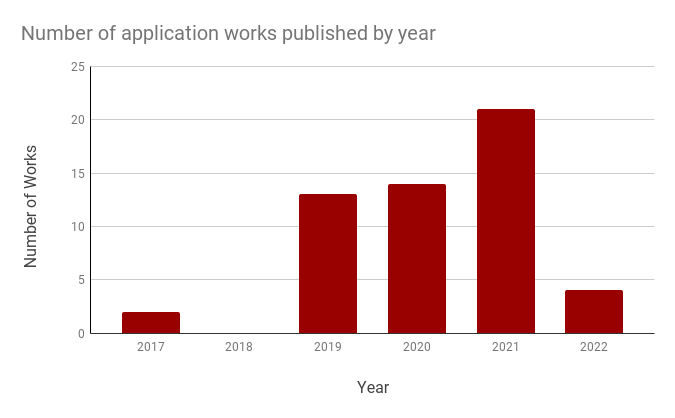
\includegraphics[width = .8\linewidth]{Figures/appl-year.png}
    \caption{Number of application papers per year. The first applications in this context were proposed in 2017, but the it was established in 2019.}
    \label{fig:appyear}
\end{figure}

After studying the works in the literature, we provide an initial overview of some information extracted from the collected data. This information aims to surround the main common aspects of the studied works. Initially, we provide an overview of how many papers were found each year. Figure \ref{fig:appyear} displays the results of this analysis.

From this result, we can initially state that the preliminary works that apply Edge AI concepts came from 2017. Nevertheless, the data indicate that the concept was actually established in 2019. After this year, the number of novel proposed applications is consistent and increased in 2021. Some Edge AI papers were already found in the first quarter of 2022.

\begin{figure}[h!]
    \centering
    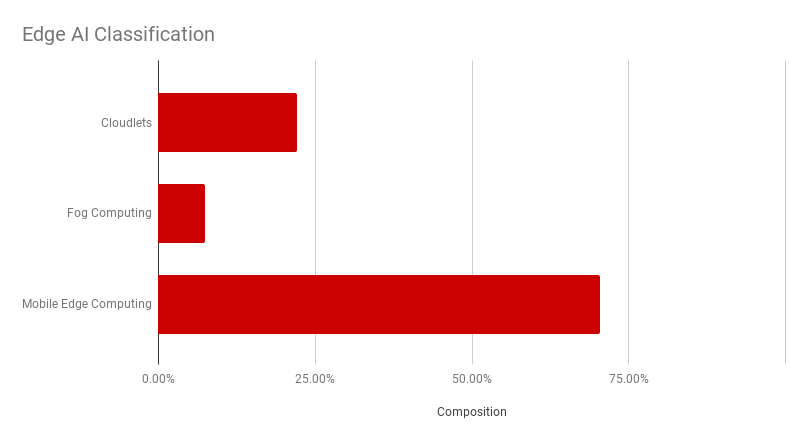
\includegraphics[width = \linewidth]{Figures/edge-classification.png}
    \caption{Contributions of each category of edge computing to the curated appliances. The majority of works apply ``Mobile edge computing''.}
    \label{fig:edgeclass}
\end{figure}

A second relevant analysis regards the edge computing classification. This section classified the works among ``Mobile edge computing'', ``Fog computing'', and ``Cloudlets''. Of the 54 curated articles, 38 applications used Mobile edge computing, 12 used Cloudlets, and four applied Fog computing. Figure \ref{fig:edgeclass} displays the classification data analysis in proportions.

\begin{figure}[h!]
    \centering
    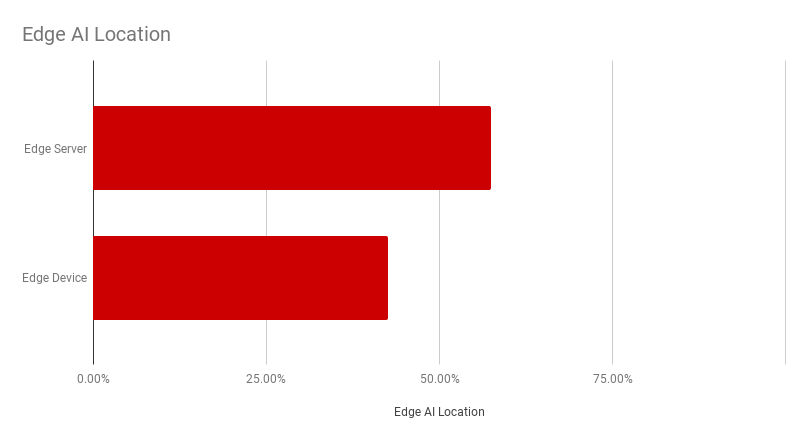
\includegraphics[width = \linewidth]{Figures/location-ai.png}
    \caption{Location of the AI algorithms. The analysis display that appliances can deploy models on edge devices or edge servers.}
    \label{fig:ailocation}
\end{figure}

Another feasible study is whether the appliances run the models in the edge devices or edge servers, according to our preliminary classification. A few more works deployed AI models on edge servers than edge devices. Nonetheless, the data is almost balanced, displaying circa 57\% of the works with AI deployed on edge servers and 43\% on edge devices. In this case, the two works that could run on both devices and servers were classified as ``Edge Device''. Figure \ref{fig:ailocation} displays these results.

\begin{figure}[h!]
    \centering
    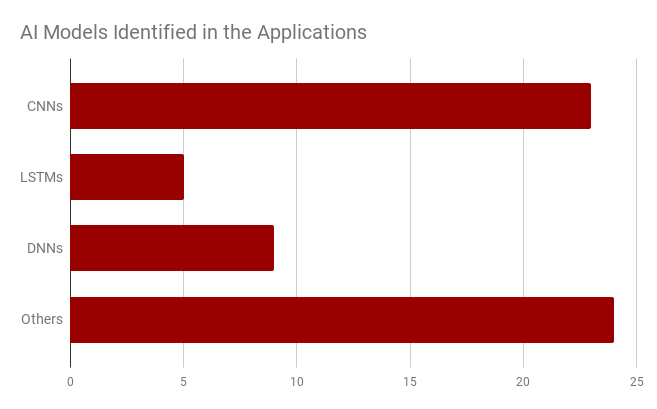
\includegraphics[width = .8\linewidth]{Figures/ai-models.png}
    \caption{AI models identified in the articles. The three individual categories that contributed the most are CNNs, LSTMs, and DNNs. Many authors identify their appliances generically as ``Machine Learning''}
    \label{fig:aimodels}
\end{figure}

Finally, we assess the models used in the studied applications. After inspecting the works initially, we decided to classify the applications among the following classes: \textbf{CNNs}, \textbf{LSTMs}, \textbf{DNNs}, and \textbf{Others/Unspecified}. The three initial classes represent the most models which were individually identified in the papers found in the literature, while the last one treats the exceptions. If a system employs more than one algorithm, all models contribute individually to the count. The results, displayed in Figure \ref{fig:aimodels}, show that CNNs are the most popular models among Edge AI applications. Also, many authors did not specify the machine learning models applied, focusing their papers on the edge computing architecture. DNNs and LSTMs had relevant individual contributions to these numbers.


%%%%%%%%%%%%%%%%%%%%%%%%%%%%%%%%%%%%%%%%%%%%%%%
\section{Edge Computing and AI taxonomies analysis}
\label{sec:taxonomiesanalysis}

After analyzing several applications, the next stage in this research is to understand how the foundation areas are organized. For this matter, we provide a study of the taxonomies in both edge computing and AI means. After this stage, we expect to extract enough information to propose an Edge AI taxonomy.

\subsection{Edge Computing Taxonomies}

Initially, we explored a few works regarding edge computing taxonomies. Finding general information in edge computing taxonomies was not easy, as most texts are focused on single areas or applications. For instance, Beck et al. \cite{beck2014mobile} focus on examining the taxonomy of mobile edge computing solutions. While his work is extensive, it refers to one single of the three main areas of Edge Computing. Thus, this work does not provide a general view of the area.

Regarding a general view of edge computing, Ahmed et al. \cite{ahmed2017bringing} display a comprehensive taxonomy of information that defines edge computing. An essential aspect of this taxonomy within the context of this work is that the authors also evaluate the same computing paradigms as presented by Khan et al. \cite{khan2019edge}, which were one of the bases of this study. The authors also generally classify the technologies among edge devices and edge servers, later using their taxonomy to evaluate the most critical enabling technologies for edge computing.

Dolui and Datta \cite{dolui2017comparison} also use the same three paradigms to classify edge computing applications. These three paradigms work as a baseline to understand the nodes' organization, nodes location, software architecture, context awareness, geographical proximity, access, and communication. This result reinforces the usage of these three paradigms as the general line to classify edge computing applications.

The analysis of these studies, combined with the previous evaluations, leads to the conclusion that a set of technologies based on edge computing should be initially evaluated according to the three computing paradigms that compose the area. The separation among cloudlets, fog computing, and mobile edge computing allows a general classification of the solutions, leading further to the AI classification.

\subsection{AI Algorithms Taxonomies}

The ways of classifying AI are broader than edge computing. For instance, Sheth et al. \cite{sheth2020taxonomy} classify AI according to the learning paradigm (supervised learning, unsupervised learning, reinforcement learning). While we understand that this will later be important to evaluate Edge AI techniques, we search for a broader classification within this work. Another example of this specificity happens in Baltru{\v{s}}aitis, Ahuja, and Morency \cite{baltruvsaitis2018multimodal}. These authors create a taxonomy of specific deep learning relevant within the Multimodal Machine Learning context.

Similarly, Talbi \cite{talbi2021machine} divides AI works according to the algorithms. They provide this classification in the context of evaluating how these algorithms can support metaheuristics. From this work, we understand that using the algorithm paradigms to classify these works is an interesting way of approaching the problem. Still, the way to perform this classification depends on the objective of the algorithms. After searching and evaluating works, we understand that the taxonomy within the AI context should consider the specificity of the desired tasks and concepts. 

\section{Edge AI Taxonomy}
\label{sec:taxonomy}

\begin{figure*}[ht!]
    \centering
    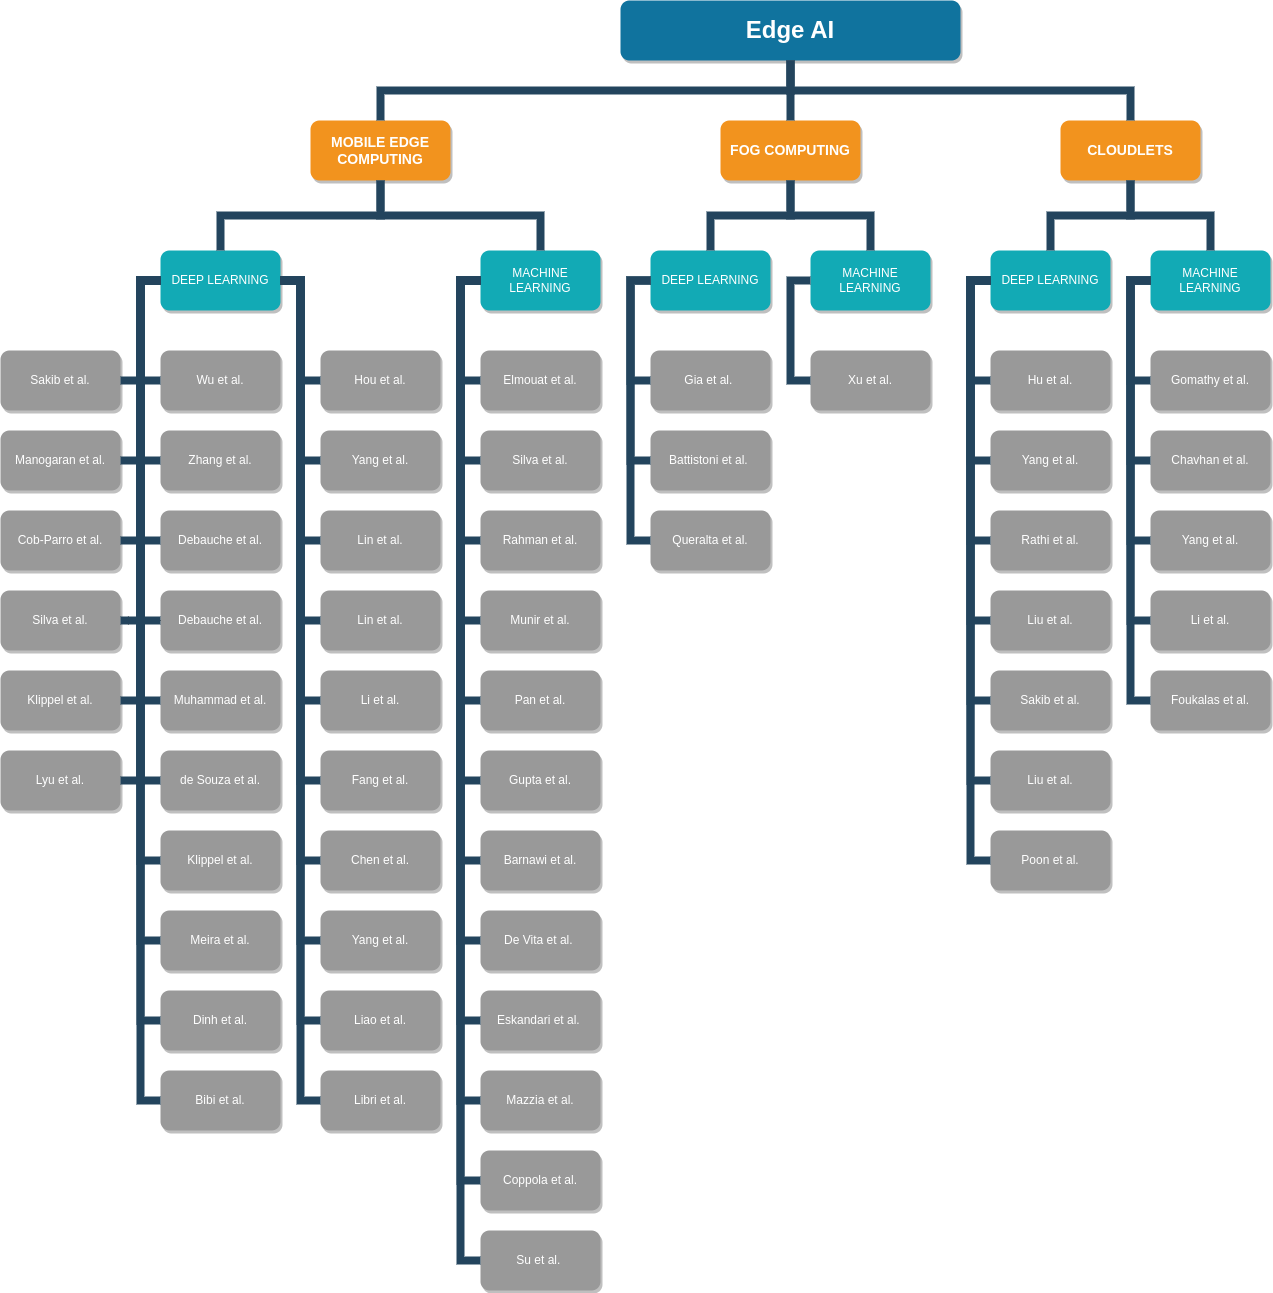
\includegraphics[width=\linewidth]{Figures/taxonomy.png}
    \caption{Classification of the works from Section \ref{sec:mapping} according to the proposed taxonomy. Each gray square is a single work evaluated in this section of the work.}
    \label{fig:taxonomy}
\end{figure*}

Given the knowledge built up to this point, we extracted enough information to propose a new taxonomy to classify Edge AI works and applications. Initially, we start with the edge computing domain, classifying the application among its classes. Then, we evaluate the application according to the AI domain.

The reviews indicate that the classification among the three main classes is adopted for the edge computing traits in both application works and taxonomies. Thus, the first layer of the Edge AI taxonomy evaluates if the works belong to \textit{mobile edge computing}, \textit{fog computing} or \textit{cloudlets} domains. This separation is efficient for dividing edge computing works while separating among edge devices or edge servers only makes sense within \textit{mobile edge computing} domain.

In the AI computing features, we initially observed several ways to separate AI algorithms. Thus, interpreting the data obtained in Section \ref{sec:mapping} was the critical aspect of defining this division. In Figure \ref{fig:aimodels}, we observe that most works use CNNs, LSTMs, or DNNs as the basis of the application. These models belong to the deep learning domain. A similar proportion of works employ other machine learning models or paradigms to employ AI on edge. Thus, we defined two classes: \textit{deep learning}, containing the applications that employ algorithms belonging to the deep learning domain, and \textit{machine learning}, encompassing the applications that employ other methods and paradigms.

In Figure \ref{fig:taxonomy}, we display the reclassification of the works presented in Section \ref{sec:mapping} according to the proposed taxonomy. We manually evaluated each work in this section according to the proposed divisions. If the works employ methods from more than one domain, including deep learning, we consider them to belong to the \textit{deep learning} classes.

What we observe in this case is that the proportions indicate by Figures \ref{fig:edgeclass}, \ref{fig:ailocation}, and \ref{fig:aimodels} were reflected in this taxonomy. Most of the works from Edge AI belong to the \textit{mobile edge computing} domain. Also, most employ algorithms belonging to the \textit{deep learning} domain. The fewest amount of applications was found regarding the \textit{fog computing} domain, while a reasonable amount was found regarding the \textit{cloudlets} domain, with a more balanced division between \textit{deep learning} and \textit{machine learning}.

Finally, we organized a taxonomic table of the displayed works for a better understanding. In Table \ref{tab:taxonomic-table}, we compiled the results displayed through Figure \ref{fig:taxonomy}. This information complements what we presented previously, working as a catalog to find works related to each area.


% Please add the following required packages to your document preamble:
% \usepackage{graphicx}
\begin{table}[h!]
\centering
\caption{Taxonomic table compiling the collected information from papers.}
\label{tab:taxonomic-table}
\resizebox{\textwidth}{!}{%
\begin{tabular}{lll}
\hline
\textbf{Paper Title} & \textbf{Edge Computing Paradigm} & \textbf{AI Paradigm} \\ \hline
Energy efficient for UAV-enabled mobile edge computing networks: Intelligent task prediction and offloading \cite{wu2020energy} & Mobile Edge Computing & Deep Learning \\
Real-time strawberry detection using deep neural networks on embedded system (rtsd-net): An edge AI application \cite{zhang2022real} & Mobile Edge Computing & Deep Learning \\
Edge computing and artificial intelligence for real-time poultry monitoring \cite{debauche2020edge} & Mobile Edge Computing & Deep Learning \\
Edge AI-IoT pivot irrigation, plant diseases, and pests identification \cite{debauche2020edge-1} & Mobile Edge Computing & Deep Learning \\
Edge Intelligence-Assisted Smoke Detection in Foggy Surveillance Environments \cite{muhammad2019edge} & Mobile Edge Computing & Deep Learning \\
Deep-Learning-Based Visual Odometry Models for Mobile Robotics \cite{de2021deep} & Mobile Edge Computing & Deep Learning \\
Conveyor Belt Longitudinal Rip Detection Implementation with Edge AI \cite{Klippel2021} & Mobile Edge Computing & Deep Learning \\
Edge Deep Learning Applied to Granulometric Analysis on Quasi-particles from the Hybrid Pelletized Sinter (HPS) Process \cite{iceis21hps} & Mobile Edge Computing & Deep Learning \\
Towards AI-Based Traffic Counting System with Edge Computing \cite{dinh2021towards} & Mobile Edge Computing & Deep Learning \\
Edge AI-Based Automated Detection and Classification of Road Anomalies in VANET Using Deep Learning \cite{bibi2021edge} & Mobile Edge Computing & Deep Learning \\
AI on edge device for laser chip defect detection \cite{hou2019ai} & Mobile Edge Computing & Deep Learning \\
An AI-edge Platform with Multimodal Wearable Physiological Signals Monitoring Sensors for Affective Computing Applications \cite{yang2020ai-2} & Mobile Edge Computing & Deep Learning \\
Implementation of Pavement Defect Detection System on Edge Computing Platform \cite{lin2021implementation} & Mobile Edge Computing & Deep Learning \\
Edge-AI-Based Real-Time Automated License Plate Recognition System \cite{lin2022edge} & Mobile Edge Computing & Deep Learning \\
Blockchain-Based Trust Edge Knowledge Inference of Multi-Robot Systems for Collaborative Tasks \cite{li2021blockchain} & Mobile Edge Computing & Deep Learning \\
\begin{tabular}[c]{@{}l@{}}Development and Validation of an EEG-Based Real-Time Emotion Recognition System Using Edge AI Computing Platform \\ With Convolutional Neural Network System-on-Chip Design \cite{fang2019development}\end{tabular} & Mobile Edge Computing & Deep Learning \\
Distributed Deep Learning Model for Intelligent Video Surveillance Systems with Edge Computing \cite{chen2019distributed} & Mobile Edge Computing & Deep Learning \\
AI-Aided Individual Emergency Detection System in Edge-Internet of Things Environments \cite{yang2021ai} & Mobile Edge Computing & Deep Learning \\
Intelligent Traffic Accident Detection System Based on Mobile Edge Computing \cite{liao2017intelligent} & Mobile Edge Computing & Deep Learning \\
pAElla: Edge AI-Based Real-Time Malware Detection in Data Centers \cite{libri2020paella} & Mobile Edge Computing & Deep Learning \\
Towards the edge intelligence: Robot assistant for the detection and  classification of human emotions \cite{sakib2021deep} & Mobile Edge Computing & Deep Learning \\
\begin{tabular}[c]{@{}l@{}}Wearable IoT Smart-Log Patch: An Edge Computing-Based Bayesian Deep Learning Network System\\ for Multi Access Physical Monitoring System \cite{manogaran2019wearable}\end{tabular} & Mobile Edge Computing & Deep Learning \\
Smart Video Surveillance System Based on Edge Computing \cite{cob2021smart} & Mobile Edge Computing & Deep Learning \\
Wearable Edge AI Applications for Ecological Environments \cite{silva2021wearable} & Mobile Edge Computing & Deep Learning \\
Deep Learning Approach at the Edge to Detect Iron Ore Type \cite{klippel2021deep} & Mobile Edge Computing & Deep Learning \\
Green Citrus Detection and Counting in Orchards Based on YOLOv5-CS and AI Edge System \cite{lyu2022green} & Mobile Edge Computing & Deep Learning \\ \hline
Edge computing and artificial intelligence for landslides monitoring \cite{elmoulat2020edge} & Mobile Edge Computing & Machine Learning \\
IDiSSC: Edge-computing-based Intelligent Diagnosis Support System for Citrus Inspection \cite{iceis21orange} & Mobile Edge Computing & Machine Learning \\
A Lossless Data-Hiding based IoT Data Authenticity Model in Edge-AI for Connected Living \cite{rahman2021lossless} & Mobile Edge Computing & Machine Learning \\
Intelligent and Smart Irrigation System Using Edge Computing and IoT \cite{munir2021intelligent} & Mobile Edge Computing & Machine Learning \\
A Wireless Multi-Channel Capacitive Sensor System for Efficient Glove-Based Gesture Recognition With AI at the Edge \cite{pan2020wireless} & Mobile Edge Computing & Machine Learning \\
Economic data analytic AI technique on IoT edge devices for health monitoring of agriculture machines \cite{gupta2020economic} & Mobile Edge Computing & Machine Learning \\
Intelligent Search and Find System for Robotic Platform Based on Smart Edge Computing Service \cite{barnawi2020intelligent} & Mobile Edge Computing & Machine Learning \\
Low-Power HW Accelerator for AI Edge-Computing in Human Activity Recognition Systems \cite{de2020low} & Mobile Edge Computing & Machine Learning \\
Passban IDS: An Intelligent Anomaly-Based Intrusion Detection System for IoT Edge Devices \cite{eskandari2020passban} & Mobile Edge Computing & Machine Learning \\
Real-Time Apple Detection System Using Embedded Systems With Hardware Accelerators: An Edge AI Application \cite{mazzia2020real} & Mobile Edge Computing & Machine Learning \\
Innovative Vineyards Environmental Monitoring System Using Deep Edge AI \cite{coppola2021innovative} & Mobile Edge Computing & Machine Learning \\
An Edge Intelligence Empowered Recommender System Enabling Cultural Heritage Applications \cite{su2019edge} & Mobile Edge Computing & Machine Learning \\ \hline
Edge AI in smart farming IoT: CNNs at the edge and fog computing with LoRa \cite{gia2019edge} & Fog Computing & Deep Learning \\
AI at the Edge for Sign Language Learning Support \cite{battistoni2019ai} & Fog Computing & Deep Learning \\
Edge-AI in LoRa-based Health Monitoring: Fall Detection System with Fog Computing and LSTM Recurrent Neural Networks \cite{queralta2019edge} & Fog Computing & Deep Learning \\ \hline
A semi-supervised learning approach for network anomaly detection in fog computing \cite{xu2019semi} & Fog Computing & Machine Learning \\ \hline
iRobot-Factory: An intelligent robot factory based on cognitive manufacturing and edge computing \cite{hu2019irobot} & Cloudlets & Deep Learning \\
AI-enabled emotion-aware robot: The fusion of smart clothing, edge clouds and robotics \cite{yang2020ai} & Cloudlets & Deep Learning \\
An edge AI-enabled IoT healthcare monitoring system for smart cities \cite{rathi2021edge} & Cloudlets & Deep Learning \\
A New Deep Learning-Based Food Recognition System for Dietary Assessment on  An Edge Computing Service Infrastructure \cite{liu2017new} & Cloudlets & Deep Learning \\
Deep Learning Models for Magnetic Cardiography Edge Sensors Implementing Noise Processing and Diagnostics \cite{sakib2021deep} & Cloudlets & Deep Learning \\
Intelligent Edge Computing for IoT-Based Energy Management in Smart Cities \cite{liu2019intelligent} & Cloudlets & Deep Learning \\
AI-doscopist: a real-time deep-learning-based algorithm for localising polyps in colonoscopy videos with edge computing devices \cite{poon2020ai} & Cloudlets & Deep Learning \\ \hline
Investigating the Spread of Coronavirus Disease via Edge-AI and Air Pollution Correlation \cite{gomathy2021investigating} & Cloudlets & Machine Learning \\
Edge Computing AI-IoT Integrated Energy Efficient Intelligent Transportation System for Smart Cities \cite{chavhan2022edge} & Cloudlets & Machine Learning \\
National Sports AI Health Management Service System Based on Edge Computing \cite{yang2021national} & Cloudlets & Machine Learning \\
Blockchain-Based Trust Edge Knowledge Inference of Multi-Robot Systems for Collaborative Tasks \cite{li2021blockchain} & Cloudlets & Machine Learning \\
Edge artificial intelligence for industrial internet of things applications: an industrial edge intelligence solution \cite{foukalas2021edge} & Cloudlets & Machine Learning \\ \hline
\end{tabular}%
}
\end{table}

% \section{Future Trends in Edge AI}
% \label{sec:futuretrends}

% After discussing the concept and classifications of Edge AI, we also provide this space with an overview of some areas that might contribute to this area's development. From our research, we understand that some critical issues connected to the future of Edge AI are 5G, 6G, Blockchain, and Federated Learning \cite{sheth2020taxonomy,fantacci2020federated,wang2019edge,nguyen2021federated,al2021survey}.

% \subsection{Edge AI, 5G, and 6G}

% 5G and 6G are the most current communication standards for broadband and wireless communications. Chowdhury et al. \cite{chowdhury2019role} state that the uprise of these technologies will enhance IoT-based solutions. Towards this aspect, Lovén et al. \cite{loven2019edgeai} envision the reduced latency of upcoming 5G and 6G networks as fundamental aspects in developing Edge AI applications. Xiao et al. \cite{xiao2020toward} present Edge AI as the missing link in the 5G communication paradigm. Furthermore, they assert that these technologies will have an essential role in implementing future 6G networks. Thus, they also recognize the importance of these technologies to future research involving these new communication paradigms. 5G and 6G present a substantial interest field to be considered when proposing novel applications involving Edge AI.

% \subsection{Edge AI in Blockchain}

% Blockchain is a composition using a set of technologies to provide secure transactions. Initially, it was developed towards cryptocurrencies, but its application raised as many processes require secure information storage and authentic transactions \cite{di2017blockchain}. This technology integrates well with some concepts within the Edge AI domain. It can be applied to improving mining and data processing in mobile edge computing, resource allocation in IoT/mobile edge computing, and content caching in vehicular networks \cite{qiu2019online,he2020blockchain,dai2020deep}, among others. Nguyen et al. \cite{nguyen2021federated} even explore its integration with the next paradigm, federated learning, within the context of mobile edge computing. These works display that integrating blockchain and Edge AI is a large field to explore in future implementations.

% \subsection{Edge AI in Federated Learning}

% Federated learning is an approach to distributing machine learning among devices within a network \cite{bonawitz2019towards}. This precedent is interesting within edge computing, where we expect to distribute computational charges among devices within a network. Some authors explore the possibility of reducing the computing offload or optimizing the training process by considering a federated learning approach \cite{wang2019adaptive,wang2019edge,ye2020edgefed,yu2021toward}. Others suggest fields of employment as vehicular networks and mobile edge computing \cite{ye2020federated,fantacci2020federated,lu2019differentially}. This perspective indicates that this area should also be explored for further implementations in future perspectives.

\section{Final Remarks}
\label{sec:conclusions}

Edge computing and artificial intelligence initially had conflicting requirements. As AI required more processing throughout time, edge computing developed mainly over hardware miniaturization and increased mobility. Nevertheless, a recent trend displayed increasing applications applying both concepts together, especially in mobile edge computing. Although other research papers survey functional aspects \cite{mendez2022edge}, applications for specific areas \cite{amin2020edge}, or even specific technologies \cite{lalapura2021recurrent}, the area lacks a general conceptualization and taxonomy.

This trend had several names up to this moment, but every one of them had similar premises of uniting edge computing with AI algorithms. Moreover, a significant number of papers describing applications in this context were published from 2019 on. To define this area, we started from the fundamental areas behind the appliances: edge computing and AI. We named this novel concept Edge AI, one of the names used to describe these appliances in the literature. 

Edge computing is divided into three main areas: cloudlets, fog computing, and mobile edge computing. Cloudlets refer to resourceful infrastructures built to provide AI closer to the end-user. Fog computing regards the distribution among heterogeneous devices and the virtualization of cloud-like services. Mobile edge computing describes more mobile and isolated infrastructure, where less powerful devices and more restricted resources are employed to provide AI.

AI can be divided in many ways. Mainly, it refers to machine learning processes where algorithms learn to solve a task from provided data. The more modern applications of machine learning are described in the literature as deep learning, having several specific algorithms in this domain. Within edge computing, AI can run in single-edge devices or as a service in edge servers. The first mode is only referred to in the mobile edge computing domain.

This information helped us create a taxonomy to classify applications described in papers from the literature. The works can belong to three edge domains: cloudlets, fog computing, and mobile edge computing. The first layer evaluates the edge computing classification. The second layer divides the AI among the deep learning domain or belonging to any other paradigm of AI. 

Finally, some of the main future trends regarding Edge AI integrate concepts like Blockchain, 5G, 6G, and Federated Learning \cite{sheth2020taxonomy,fantacci2020federated,wang2019edge,nguyen2021federated,al2021survey}. Future works can explore these aspects as the ground for further investigation. Also, as mobile edge computing contains the most developed area among these domains within Edge AI, it requires further investigations and classifications on its own, possibly as a ``Mobile Edge AI'' concept.

\cleardoublepage